\documentclass{llncs}

\usepackage[utf8x]{inputenc}
\usepackage{graphicx}
\usepackage{ctable}
\usepackage{tabularx}
\usepackage{subfig}

% TODO: fixa en grammatiskt korrekt titel :)
\title{Performance measurements on open source enterprise service bus}
\author{Joakim Olsson \inst{1} \and Johan Liljegren\inst{1}}

\institute{
	Blekinge Institute of Technology \\
	\email{laggmonkei@gmail.com}, \email{datanizze@gmail.com}
}

\hyphenation{}

\begin{document}
\maketitle
\begin{abstract}
Hola!
\end{abstract}

\section{Introduction} % TODO: add references
% Introduction sets focus for thesis and make reader motivated to continue reading. to do that you have to clearly explain what's being investigated, why it is relevant and what value the thesis gives to the world.

Since the dawn of software engineering we have come a long way in developing applications and platforms. The leaps forward has been greatly beneficial for everyday tasks but since more and more of these applications and platforms needs to communicate with each other it has become clear that the industry had not kept up with integrating platforms. Enter the Enterprise Service Bus (ESB). To address these integration issues terms like Enterprise Application Integration (EAI) and Service Oriented Architecture (SOA) have been visualized. The ESB is a ``next step'' in this direction, taking what's good from SOA and EAI to bring a complete platform for integration.

Where early manual integration between different platforms (often referred to as ``independent islands of computing'') was done by point to point integration, that is, for each new platform to integrate all existing platforms had to build separate interfaces to communicate with the new one. This is a very cumbersome way to do it resulting in messy integration with a lot of dependencies in the end. This type of integration is referred to as ``spaghetti code'' since connections are made from everything to everything. This is where the ESB comes in. The ESB acts a mediator, translator and monitor amongst many things. The main task for the ESB is to step in and take over communications between all involved platforms. This is done by changing the involved platforms so they connect to the ESB and only to the ESB \cite{Sanjay2011}. The main advantages of this is that the esb takes care of where to send data between the platforms making the platforms agnostic to what to send and where, they just send it to the ESB and the ESB takes care of forwarding it to the right destination with the right data at the right place in the right language.

The research focus will be on testing a number of ESB solutions' performance in the most essential tasks a ESB provides. The expectations of the outcome is to give a clear overview of the most popular ESBs' performance at the latest versions currently available.

When choosing an ESB to use a lot of parameters needs to be filled, ease of use, documentation, features and performance is a couple of things needed to make an educated decision what to use. This thesis focuses on performance since there are no current and unbiased resources about the most popular ESBs' performance.

% - problem definition: its nature and scope, why this problem? why is it important? (review relevant literature)
The nature of this thesis is to clearly define tests and results of what current ESBs have to offer in the area of performance. This was chosen since the performance of an ESB plays a mayor role in perceived overall value of an ESB since its job is broad and it handles just about every call between integrated platforms. This merges well with the aims of the thesis, which is to get a grip of current ESBs performance and to evaluate what already exists and how relevant that is

% - method of investigation: why this method?
The chosen method of investigation is to create an environment where tests can be performed, singling out performance differences in the different ESB solution offerings.
We will review literature available on the Internet in order to get a good understanding of the current body of knowledge and ascertain a need for increasing that body of knowledge. This also allows us to review how previous performance measurements have been done in this field of software design which will ensure that our test suite does not deviate or alienate previous research as well as has a somewhat well anchored position in the current software design community.


% - expected outcome: value and intended audience
The expected outcome of this thesis is to give a defined test bed with performance results from a controlled test environment for the involved ESB solutions.

% - limitations (avgränsningar)
%\subsection{Limitations}

% - thesis overview: what is presented in the following chapters and in what order
TODO: thesis overview: easier to do when we have some content to describe.
% Vi får väl fixa här när vi skrivit lite mer

\section{Background}
\label{sec:background}
% used to explain and present concepts and terms important to understand the thesis... alltså bakgrundsinfo om integration, esb, xml, xpath osv.
% Also used to further explain problem/issue that we want to investigate and motivate importance of by f.e. showing what are the gaps in the currently available body of knowledge and that you are intending to fill in some of those gaps with knowledge gathered from our research.

% should contain the following parts:
% detailed information on the background concepts necessary to understand and evaluate your results - aka ge tillräckligt med info för att någon som inte alls är insatt så de kan förstå sisisisisen.
% An overview of the related literature and state-of-the-art research in order to identify the gap and motivate the need for our research.

Enterprise Service Buses (ESB) provides a platform for integration, connecting existing platforms and products with familiar protocols \cite{falko07} . Before integration became an integral part of developing systems these now integrated parts where operating on its own without any interaction with other platforms/products. This can be viewed as ``independent islands of computing''. The ESBs task is to bring communication between these islands thus integrating them.

ESBs are pivotal in software integration and are becoming extremely important in company software solutions and infrastructures, future and ancient alike \cite{fenner03}.

As such it is very important to accurately and repeatedly measure the performance of integration solutions available. 
There are currently several open source options available \cite{mehta11} and the current body of knowledge regarding their different performance aspects is severely lacking. 

% {2-3 paragraphs giving more detailed background. Should answer: What has been done by others in this area? What is our current knowledge?}

There has been some measurements and benchmarks done by the producers of the ESBs however these measurements have always been in favor of the ESB produced by the company making the measurements. 
Impartial performance measurement are especially lacking, there are several reports made by the producers of some solutions \cite{Perera07,mulevsjboss,mulevsglassfish,mulevsservicemix,mulesoft08}.
There has been some research done in the area \cite{Sanjay2011} however the number of ESB's tested are quite limited when compared to the most up to date list of popular ESBs \cite{mehta11}.

Most importantly they do not explicitly declare what versions they are using in their tests which makes their results hard to reproduce. 
Judging by the dates on which their paper was completed it is clear that all the ESBs that they use have received major upgrades which makes it even more important to produce new measurements.

% {1 paragraph detailing the gap in our current knowledge. Should answer: What is missing in our current knowledge? What is the main purpose of doing this project? Overall, what will we do?}
The main purpose of this thesis is to increase the knowledge of differences between modern open source ESBs. 
This will hopefully lead to it being easier to further develop these software products and make it easier for end users to compare and evaluate based on their specific needs.


\section{Research question and research design}
%Chapter 3 – Research questions and research design
The research questions are as follows: 
\begin{itemize}
	\item RQ1: How accurate and up to date is our current knowledge in the academic world, what tests has been done and how/what did they measure?
	\item RQ2: How accurate and up to date is our current knowledge in the industry, what tests has been done and how/what did they measure?
	\item RQ3: What are core functionalities of an enterprise service bus?
	\item RQ4: Is it possible to produce a testing framework that provides a foundation for future testing in a transparent and unbiased way?
\end{itemize}
%Present clearly how the research questions will be answered. Some of the questions will be answered through the literature review, some through the experiment/interview/survey and some through both.
RQ4 will be answered through experiments and measurements while RQ1-3 will be answered through the literature review. 

%Present the design of your literature survey:
%How did you conduct the literature search? 
The survey design consisted of searching the different search engines listed below with the listed search strings. \\

{\bf Search engines used:}
\begin{itemize}
	\item IEEE Xplore
	\item Google
	\item Google Scholar
	\item BTHs general search engine for documents
\end{itemize}

{\bf Search strings used (and combined):}
\begin{itemize}
	\item ESB
	\item Enterprise Service Bus
	\item Enterprise Application Integration
	\item Integration
	\item Integration measurement
	\item Integration comparison
	\item Mule esb
	\item WSO2
	\item Testing
\end{itemize}

During the literature survey abstracts were read and if the abstract suited our criteria (Evaluations of open source ESBs, performance measurements, ESB comparisons amongst others) a quick look through the actual content to see if the abstract did indeed sum up the content in a fair way. If then the quick view through the paper gave any value it was read more thoroughly and then added to the list of accepted papers to use in this thesis.


%Here you should describe in detail how the experiment will be conducted, which valuables will be measured, How the experiment environment will be set up and controlled. 

\section{Testing framework}
This testing framework aims to answer RQ3. The goal is to produce a transparent and sound way of testing core functionality \cite{lit review} performance of any ESB. 
We have gathered much inspiration from Sanjay \cite{Sanjay} regarding what measurements and tests that should be performed however the focus of our effortsis to provide source code and transparency in order for the tests to be repeatable as well as having the ability to discuss how to improve testing.

\subsection{Measurements}
This section will describe what metrics will be collected and why.\\

\begin{tabular}{| c | l |}
	\hline
	\multicolumn{2}{|c|}{Metrics captured} \\
	\hline
	Client & Response time and throughput \\ \hline
	ESB & CPU and RAM \\ \hline
	Web service &  CPU \\ \hline
\end{tabular} \\

Computer specifications \\

\begin{tabular}{| c | l |}
	\hline
	Component & Specification \\ \hline
	CPU & Intel Core i7 920 @ 2.67GHz  \\ \hline
	RAM &  6,00 GB Triple-Channel DDR3 @ 533MHz (7-7-7-20) \\ \hline
	Network &  Intel(R) 82567LM-2 Gigabit Network Connection \\ \hline
	Motherboard &  Intel Corporation DX58SO (J1PR) \\ \hline
	Graphics &  256MB GeForce 7600 GS (MSI) \\ \hline
	Hard Drive &  488GB Western Digital WDC WD5001AALS-00L3B2 ATA Device (SATA) \\ \hline
\end{tabular} 
\subsubsection{Response time}
The amount of time elapsed since a request was sent to the time a response was received. 
The response time is measured because this is what a single user will be affected by the most, if the response time is very low the user will perceive the system as very fast and vice versa if the response time is too high.
\subsubsection{Throughput}
Amount of successful transactions performed per second (tps). A transaction is counted as successful if the response matches the expected values.
The value of throughput lays in how many users the system can serve in a single point of time. If the throughput is high the system will be able to handle many simultaneous users making the system efficient at handling a high load.



Response time and throughput are the most interesting numbers to investigate as they are very important for end users and systems. The more users a system can handle and the faster it does so the higher value the system will get in terms of scalability and performance per processing unit which in turn equals a lower operating cost where the system is able to handle a high amount of users whilst keeping the costs down.
CPU and RAM data will be measured in order to be able to make sure no hardware limitations occur during testing. The CPU on the web service is only collected to make sure that it doesn't act as a bottleneck while testing. Although this might not be the case in real world scenarios the aim is not to cap any hardware limitations because that would not give fair test results since the hardware would limit the performance of the system being tested and since the framework is supposed to give the involved system(s) free roam hardware limitations would be in straight contrast to what the framework is about.

\section{Test walktrough}
The tests described below are aimed at measuring the very basic roles of any ESB. 
The tests are very simple with the specific goal of producing a baseline for future tests. 
These basic tests have been chosen since anyone with the development knowledge of an ESB should be able to produce an ESB project capable of delivering a runnable project which exposes these basic funtionalities.

\subsection{Pure throughput}
No manipulation of the data will be done by the ESB in this test. The ESB will purely forward all request to the target web service as fast as possible. 
This test could simulate a service where the ESB exposes an inbound endpoint for other system to connect to, modularizing which service is running in the background thus giving a separation of concerns where the requesting client does not have to know about the responding web service, just that a web service is made available by the ESb.
A comparative test can be performed here as well and that is to not use the ESB which will show what performance impact the ESB adds. 

\centerline{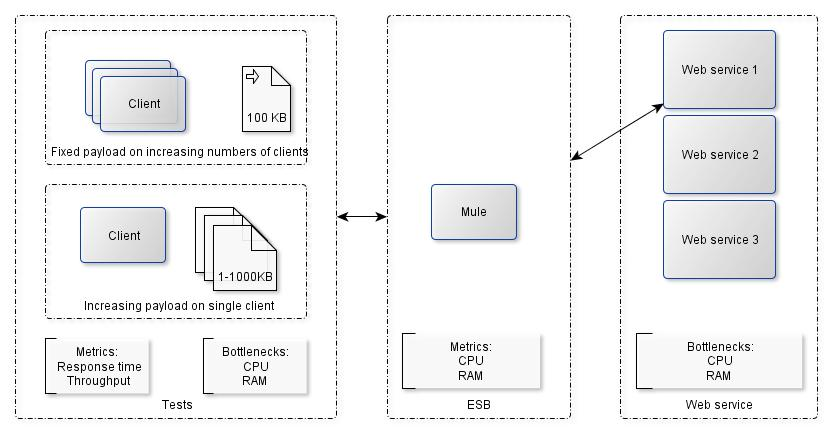
\includegraphics[scale=0.43]{img/direct_proxy}}

\subsection{Routing}
In this test the ESB will, depending on the context of an incoming request from the Client, send the request to an appropriate web service which will append some data and return the request to the ESB which will send the response to the Client.
This represents the ability to have several systems behind an ESB all showing the same front to the outside.
This test is deemed basic because it is what an should do, separate the systems integration with each other, stepping in as a ``middle-man'' directing requests on behalf of the systems being integrated making the need for changing the systems minimal and just focus on the ESB. 
A test like this could simulate a load balancer where the ESB is a front for two or more systems each running an instance of the same service. Another thing this could simulate is different systems handling different (but similar) data, for example one system behind the ESB is handling user registrations and another one is handling user logins. The ESB can then look at the request payload and decide what user interaction is happening and thus mediate the request to the appropriate system.

\centerline{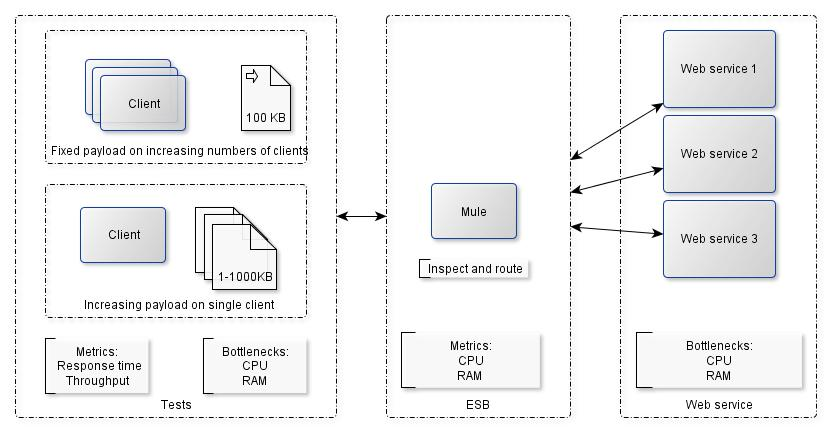
\includegraphics[scale=0.43]{img/Routing}}
\subsection{Message transformation}
The ESB will convert an incoming request to a different format and send it to a web service which will append some data and return the request to the ESB which will transform it back into the format the Client originally sent it.
Transformation is a huge deal for any ESB since two systems to be integrated probably will not speak the same language (XML, json etc) and even if they do they may not have the same format. Of course the systems need to be able to communicate with each others, without an ESB this could become cumbersome since all involved systems would have to be changed in order to understand what the others where saying, just imagine an old system written in COBOL or Assembler and making it communicate with a new system like a web service using REST \cite{whatisrest}. Integration like this cost both money and time and probably won't be future friendly with regards to maintenance.
This could make an ESB invaluable since the ESB would take care of receiving the incoming request in one format, decide where the request is to be sent, transform it to a format which the receiving system can understand, get a response back and transforming it to a format the original system which sent the request will understand.

\centerline{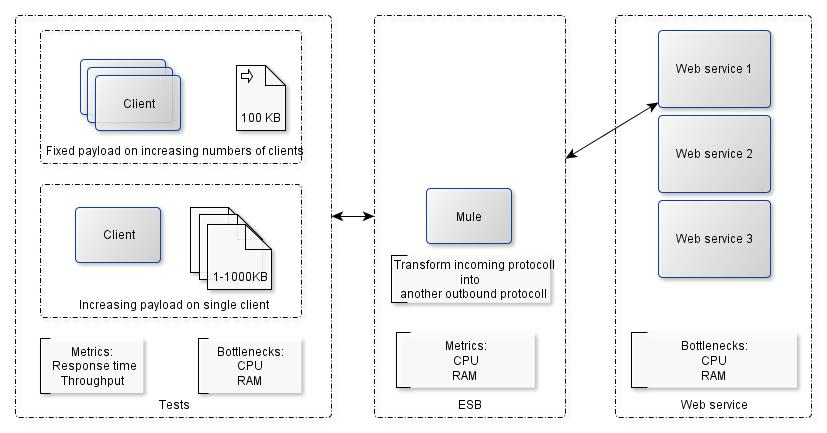
\includegraphics[scale=0.43]{img/transformation}}
\subsection{Artifacts and tools}
\begin{itemize}
	\item Client: Grinder \cite{whatisgrinder, kod}
	\item ESB: Mule \cite{whatismule, kod}
	\item Web service: Jax-WS \cite{whatisjaxws, kod}
	\item OS: Windows 7, 6.1.7600 build 7600
\end{itemize}

\subsection{Hardware setup}
In order to minimize the amount of factors that interfere in the tests we consider having at least three similar state of the art computers, connected to a high-speed network, essential.
It might not be of the greatest importance that the computers are state of the art but in order to not reach a hardware ceiling while testing, such machines are recommended. 
What's most important is that one computer is designated to run ESBs, one is designated to generate traffic(called Client) while the others are simple servers responding to the traffic generated (called Web service). 

% TODO: fixa en lista över hårdvaran (CPU,RAM,HDD osv osv)

This separating and designating of roles to machines minimizes different hardware affecting test results as the same machines perform the same roles in all tests and the only thing changed is the ESB. 

It also means that if other machines are used in other tests the data produced can be compared to ours and as such validate the data or identify faults in the tests. 
This validation can be done in two ways. 
First is to run the same software versions and compare the results. 
They should be similar deviating only in magnitude. The second is if using a newer or old software version the values when put in a graph will either have the same shape or show areas in which performance has changed, 
if it is the same shape but the magnitude is higher then that is most likely caused by faster machines being used and vice versa if its the same magnitude except in certain areas then that shows an improvement in the software.

\subsection{Variables and variable control}
No limitiations has been forseen except for hardware and notwork.
Hardware and network loads should be monitored so they are not close too 100\% as that would mean there is a major bottleneck present. 
All involved computers a run with the same operating system.
\subsection{Experiment schedule and execution sequence}
The three tests have two different focuses. First is to test scalability with an increasing amount of simulated clients (1, 20, 40, 80, 160) sending concurrent requests. 
The other is to test load-handling where a single client will send varying sizes of payload, 1KB, 50KB, 100KB, 500KB and 1MB.
\subsection{Validity threats}
This section discusses different validity threats.
\subsubsection{Different operating systems}
%Different operating system will effect test results 
%TODO säkerställ att unix inte påverkar resultaten nämnvärt
kan påvera men vi kommer att köra testerna på lite olika system så vi har ett hum om vilka förändringar det innebär i datan.
\subsubsection{Different hardware}
%TODO kör testerna en gång på /// så vi inte påverkas för mycket av hårdvara
see "different operating systems"
\subsubsection{Inefficient code}
We are not expert in the various programming languages and systems used to perform these tests and as such our code might be inefficient and even wrong. Inefficient code is not a problem as long as the same code is used in all tests. Erroneous code however is unmaintainable code and as such will require too be changed in the future and that will most likely affect the test results and test history. 
The possibilities of erroneous code has been limited by focusing the tests on very simple and basic functionality that doesn't require expert knowledge of the ESB in order to get results.
By actually providing the source code we have opened up the possibility for improvements and additions of more advanced tests which we feel is extremely important for a consistent testing framework used in academia and industry.

\label{sec:method}
\section{Literature review results}
\label{sec:litrev}

The literature review has focused on what the academic world knows and what the industrial world knows and as such we will present them separate and then conclude.

% - Present the papers that you have identified as your information source. Describe them, what type of papers they are, from what period; what do they have in common etc.
\subsection{Academia}
"Enterprise Service Bus"\cite{falko07} by Falko Menge is a paper that explains the fundamentals of an ESB as well as introduces Mule with an example. Published in 2007 its example has become obsolete and outdated however the fundamentals still hold true as seen by later papers such as "Research of Enterprise Application Integration Based-on ESB" \cite{Jieming2010} by Jieming Wu and Xiaoli Tao as well as "Integration of Distributed Enterprise Applications: A Survey" \cite{HeIntegration} by Wu He and Li Da Xu these are papers that focus on describing the history and evolution of software integration. They were published in 2010 and give an in depth view on how an ESB  operates.


"An Interoperability  Study  ofESB for C4I  Systems " \cite{Alghamdi2010} by Abdullah Alghamdi, Muhammad Nasir, Iftikhar Ahmad and Khalid A. Nafjan and  "Adopting and Evaluating Service Oriented Architecture in Industry" by Khalid Adam Nasr, Hans-Gerhard Gross and Arie van Deursen are papers showing the importance of ESBs in the modern world. Published in 2010 they represent a modern necessity for ESBs in industry.


"Service-Oriented Performance Modeling the MULE Enterprise Service Bus (ESB) Loan Broker Application " \cite{Brebner2009} by Paul Brebner is a paper from 2009 going trough how the author builds a integration solution and tests it, however the author tests the entire solution which isn't general enough for what we consider a performance test of an ESB. The author does however discuss some aspects of testing that are vital such as how and where to measure.

"Evaluating Open Source Enterprise Service Bus" \cite{Garcia2010} by F. J. García-Jiménez and M. A. Martínez-Carreras, A. F. is the first paper found that performs a performance test however the test is limited in variation and magnitude. The paper was published in 2010 which makes the test outdated since all ESBs in the test has received major updates since 2010.


"Enterprise Service Bus: A Performance Evaluation" \cite{Sanjay2011} by Sanjay P. Ahuja and Amit Patel  is the only paper found that performs a performance test directly aimed at the different ESBs with a varied test suite and varied measurements. Published in 2011 it is also the most recent paper found however all ESBs tested has received major updates since then and as such needs to be retested.

% - Present your approach for analyzing selected papers in order to find concepts/topics/data/events/experiences that are relevant for answering your research questions
The above papers has as per the literature review design first been identified by its abstract and then read in detail to find those that describe the concept of an ESB and those that test ESBs in various ways. We have selected papers according too three topics. First is a basic ESB understanding and explanation in order to assert an understanding of how an ESB works and its history. We consider this important since in order to understand the importance of a software it is imperative one has a firm understanding of its fundamentals. After that fundamental has been established we concentrated on papers that shows a use for ESBs in real world industry and organizations. This in order to convey a sense of the use and importance of ESBs and research concerning it.
Finally we focused on papers that performs any kind of tests in order to establish an understanding of the current body of knowledge in the academic world. Most important were papers testing ESBs and not solutions, performance and not overall feature checks.

% - Present and describe the findings from your literature survey and their relation to your research questions
% - Discuss your findings and conclude literature survey results.

The fact that we have only found two papers performing tests is a very clear indication that the academic world does not perform performance test/analysis on ESBs. The ones we have found are all considered old in a rapidly changing world and all but one performs a test that we find adequate.


\subsection{Industry}

First of all we found an article\cite{mehta11} which listed what the author thought were the best ESBs available in 2011. This is important as it provides us with a list of ESBs that we can pick and choose from when selecting candidates for our performance test and it provides us with focus points on where to start searching for performance tests performed by ESBs themselves. This is also the most recent article of its kind aswell as the largest that we found.

In 2007 WSO02 started with a series of three performance tests against other leading ESBs \cite{Perera07,Perera07R2,Perera07R3}. In the third they compare against Mule ESB which in turn responds with a performance test of their own \cite{mulesoft08}. The tests performed in these tests are sensible and aim to present an understanding of how the different ESBs perform while doing basic tasks. A problem however is that the results are from 2008 and later which mean that they are extremely out of date and maybe even more important is that they are biased.


Mule has published a few articles that are not performance test but instead some kind of sales comparison with a number of other ESBs\cite{mulevsjboss,mulevsglassfish,mulevsservicemix}.

And finally we have read the Forrester report \cite{forrester11} from 2011 which is a industry initiated report that further visualizes the need for ESBs in modern software development, It is not performance oriented and includes non open-source ESBs.

The industry seem to have a good understanding of how to test their products however they do not seem to update their results and as such they hold little value.

\subsubsection{Core ESB functionality}
There are a few different views on what the core functionality of ESBs are however they all seem to contain three similar functions. Those functions are proxying, routing and mediation. 

\begin{description}
	\item[Proxying] \hfill \\
			The ability to 
	\item[Routing] \hfill \\
			The ability to based on incoming requests route the request to the correct recipient.
	\item[Mediation] \hfill \\
			The ability to transform incoming requests from one message protocoll(SOAP, REST, JSON) into another protocoll that the recipiant requires.
\end{description}

\subsubsection{Literature review conclusion}

It is apparent that the academic world is seriously lacking any kind of performance tests regarding the ESB field of software engineering. We found one paper\cite{Sanjay2011} that produced a test suite with a good enough scope and focus. It is however becoming out dated due too the fast pace of the industry and there are no collaborating papers supporting the results produced and as such it by itself hold little value. The industry has made a good effort in providing sensible tests that focuses on the basic performance but those results are old and outdated. 
It is therefore our conclusion in regards to R3 that the current body of knowledge is very inaccurate and outdated. We believe that \cite{Sanjay2011} and \cite{Perera07,Perera07R2,Perera07R3,mulesoft08}still holds some merit in regards to how tests should be performed but the actual results they have produced have not been confirmed by other independent sources and are now too old for reproduction.

\section{Performance test}
%TODO: needs further indepth analysis 
It is important to define what tests are done in our references as well as define what we would like to define as a sensible testing routine.
\subsection{What is a performance test?}

measurements conducted on machines running software while the software is undergoing a controlled amount of traffic/load with the goal to find breakpoints in the software and hardware. the hardware should remain the same throughout the test in order to minimize errors in measurements and the machines producing the traffic/load should also be controlled and verified that they produce the correct load. 
\subsection{Test walk trough}
	\subsection{Mule ESB}
	\subsection{WSO2}
	\subsection{Servicemix}
	\subsection{OpenESB}
	\subsection{UltraESB}

\section{Data synthesis and answer to research questions}
\section{Conclusion}

\bibliographystyle{ieeetr}
\bibliography{refs}
\end{document}

